% Free range VHDL
% Authors: Bryan Mealy, Fabrizio Tappero
% Date: May, 2012
% URL: freerangefactory.org
% (C) 2013 B. Mealy, F. Tappero
%
% !TEX root = master.tex
%
% Solutions for the exercises
% Authors: Stefan Gänsler
\chapter{Exercises Solutions}
This chapter provides example solutions for the exercises in this book. Be aware that solutions here are not always the only solution. W we wanted to give you a recommendation for example solutions so you can compare with your answers.

\section{Solutions \ref{vhdl_design_units_exercises}~\nameref{vhdl_design_units_exercises}}
\begin{my_num_list}
	\item \textit{What is referred to by the word bundle?}\\
	``Bundle'' is used to refer to a set of similar signals. These are commonly referred to as ``bus signals'' in computer lingo.

	\item \textit{What is a common method of representing bundles in black-box diagrams?}\\
	\begin{minipage}{\linewidth}
	    \centering
		\begin{tikzpicture}[x=1mm,y=1mm,line width=0.8pt,scale=0.8,framed]
		%\draw[help lines] (0,0) grid (50,50);
		% BOX
		\draw (20,0) rectangle (37,8) node[midway]{};
		% INPUTS
		\small
		\node (hide) at (0,10) {}; % just to expand background
		\node (a) at (20,0) {}; % this is the reference point
		\draw [latex-] ($(a)+(0,4)$) -- ++(-10,0) node[left]{bundle\_input} node[pos=0.4,above]{3} node[pos=0.7]{/};
		% OUTPUTS
		\draw [-latex] ($(a)+(17,4)$) -- ++(10,0) node[right]{bundle\_output} node[pos=0.7,above]{8} node[pos=0.4]{/};
		\end{tikzpicture}
	\end{minipage}

	\item \textit{Why is it considered a good approach to always draw a black-box diagram when using VHDL to model digital circuits?}\\
	First, it simplifies the design from a systems standpoint. Examining a circuit diagram containing appropriately named black boxes is much more understandable than staring at a circuit containing a countless number of logic gates. Second, the black-box approach allows for the reuse of previously written code.

	\item \textit{Write VHDL entity declarations that describe the following black-box diagrams [...]}\\
	\noindent
	\begin{minipage}{1\linewidth}
		a)
		\begin{lstlisting}[]
		entity sys1 is
		port (
			a_in1, b_in2, clk, ctrl_int   : in  std_logic;
			out_b                         : out std_logic;
		end sys1;
		\end{lstlisting}
	\end{minipage}

	\noindent
	\begin{minipage}{1\linewidth}
		b)
		\begin{lstlisting}[]
		entity sys2 is
		port (
			input_w, clk     : in  std_logic;
			a_data, b_data   : in  std_logic_vector(7 downto 0);
			dat_4            : out std_logic_vector(7 downto 0);
			dat_5            : out std_logic_vector(2 downto 0);
		end sys2;
		\end{lstlisting}
	\end{minipage}

	\item \textit{Provide black-box diagrams that are defined by the following VHDL entity declarations [...]}\\
	a)\\
	\noindent
	\begin{minipage}{\linewidth}
		\centering
		\vspace{5pt}
		\begin{tikzpicture}[x=1mm,y=1mm,line width=0.8pt,scale=0.8,framed]
			%\draw[help lines] (0,0) grid (50,50);
			% BOX
			\draw (20,5) rectangle (37,35) node[midway]{ckt\_c};
			% INPUTS
			\small
			\node (hide) at (0,35) {}; % just to expand background
			\node (a) at (20,-2.5) {}; % this is the reference point
			\draw [latex-] ($(a)+(0,35)$) -- ++(-10,0) node[left]{bun\_a} node[pos=0.4,above]{8} node[pos=0.7]{/};
			\draw [latex-] ($(a)+(0,30)$) -- ++(-10,0) node[left]{bun\_b} node[pos=0.4,above]{8} node[pos=0.7]{/};
			\draw [latex-] ($(a)+(0,25)$) -- ++(-10,0) node[left]{bun\_c} node[pos=0.4,above]{8} node[pos=0.7]{/};
			\draw [latex-] ($(a)+(0,20)$) -- ++(-10,0) node[left]{lda};
			\draw [latex-] ($(a)+(0,15)$) -- ++(-10,0) node[left]{ldb};
			\draw [latex-] ($(a)+(0,10)$) -- ++(-10,0) node[left]{ldc};
			% OUTPUTS
			\draw [-latex] ($(a)+(17,32.5)$) -- ++(10,0) node[right]{reg\_a} node[pos=0.7,above]{8} node[pos=0.4]{/};
			\draw [-latex] ($(a)+(17,22.5)$) -- ++(10,0) node[right]{reg\_b} node[pos=0.7,above]{8} node[pos=0.4]{/};
			\draw [-latex] ($(a)+(17,12.5)$) -- ++(10,0) node[right]{reg\_c} node[pos=0.7,above]{8} node[pos=0.4]{/};
		\end{tikzpicture}
	\end{minipage}
	b)\\
	\noindent
	\begin{minipage}{\linewidth}
		\centering
		\vspace{5pt}
		\begin{tikzpicture}[x=1mm,y=1mm,line width=0.8pt,scale=0.8,framed]
			%\draw[help lines] (0,0) grid (50,50);
			% BOX
			\draw (20,5) rectangle (37,40) node[midway]{ckt\_e};
			% INPUTS
			\small
			\node (hide) at (0,40) {}; % just to expand background
			\node (a) at (20,-2.5) {}; % this is the reference point
			\draw [latex-] ($(a)+(0,40)$) -- ++(-10,0) node[left]{RAM\_CS};
			\draw [latex-] ($(a)+(0,35)$) -- ++(-10,0) node[left]{RAM\_WE};
			\draw [latex-] ($(a)+(0,30)$) -- ++(-10,0) node[left]{RAM\_DE};
			\draw [latex-] ($(a)+(0,25)$) -- ++(-10,0) node[left]{SEL\_OP1} node[pos=0.4,above]{4} node[pos=0.7]{/};
			\draw [latex-] ($(a)+(0,20)$) -- ++(-10,0) node[left]{SEL\_OP2} node[pos=0.4,above]{4} node[pos=0.7]{/};
			\draw [latex-] ($(a)+(0,15)$) -- ++(-10,0) node[left]{RAM\_DATA\_IN} node[pos=0.4,above]{8} node[pos=0.7]{/};
			\draw [latex-] ($(a)+(0,10)$) -- ++(-10,0) node[left]{RAM\_ADDR\_IN} node[pos=0.4,above]{10} node[pos=0.7]{/};
			% OUTPUTS
			\draw [-latex] ($(a)+(17,25)$) -- ++(10,0) node[right]{RAM\_DATA\_OUT} node[pos=0.7,above]{8} node[pos=0.4]{/};
		\end{tikzpicture}
	\end{minipage}

	\item \textit{The following two entity declarations each contain two of the most common syntax errors made in VHDL. What are they?}

	\noindent
	\begin{minipage}{1\linewidth}
		a)
		\begin{lstlisting}[]

		entity ckt_a is
		port (
		J,K : in  std_logic;
		CLK : in  std_logic; -- last semicolon was missing
		Q   : out std_logic); -- last semicolon has to be outside the bracket
		end ckt_a;
		\end{lstlisting}
	\end{minipage}

	\noindent
	\begin{minipage}{1\linewidth}
		b)
		\begin{lstlisting}[]

		entity ckt_b is
		port (
		mr_fluffy   : in  std_logic_vector(15 downto 0);
		mux_ctrl    : in  std_logic_vector(3 downto 0);
		byte_out    : out std_logic_vector(3 downto 0)); -- closing bracket for port was missing, semicolon has to be written after closing bracket
		end ckt_b;
		\end{lstlisting}
	\end{minipage}

\end{my_num_list}

\section{Solutions \ref{vhdl_programming_paradigm_exercises}~\nameref{vhdl_programming_paradigm_exercises}}
% TODO: All solutions for all exercises

\section{Solutions \ref{standard_models_in_vhdl_architectures_exercises}~\nameref{standard_models_in_vhdl_architectures_exercises}}
% TODO: All solutions for all exercises

\section{Solutions \ref{vhdl_operators_exercises}~\nameref{vhdl_operators_exercises}}
% TODO: All solutions for all exercises

Basic source code to start with for solution:
\begin{lstlisting}[]
library IEEE;
use IEEE.std_logic_1164.all;
use IEEE.numeric_std.all;

entity FPGA_Chapter_6 is
port
(
	-- Input ports
	user_pb    : in std_logic_vector (0 to 2);
	clkin_50   : in std_logic;


	-- Output ports
	user_led   : out std_logic_vector (0 to 3) := "1111"

);
end FPGA_Chapter_6;

architecture archi of FPGA_Chapter_6 is
	signal output     : std_logic := '0';
	signal S, D, R, Q : std_logic := '0';
	signal clk_1Hz    : std_logic := '0';

begin

	process(clkin_50) is
		variable clk_counter : integer := 0;
	begin
		if(rising_edge(clkin_50)) then
			clk_counter := clk_counter + 1;

			if(clk_counter mod 25000000 = 0) then
				clk_1Hz <= NOT clk_1Hz;
			end if;

			if(clk_counter = 50000000) then
				clk_counter := 0;
			end if;
		end if;
	end process;

	S <= NOT user_pb(0);
	D <= NOT user_pb(1);
	R <= NOT user_pb(2);

	-- Chapter 6 T Flip-Flop
	process(clk_1Hz) is
	begin
		if(S = '1') then
			Q <= '1';
		elsif(R = '1') then
			Q <= '0';
		elsif(rising_edge(clk_1Hz)) then
			-- Q <= D;
			if(D = '1') then
				Q <= NOT Q;
			end if;
		end if;
	end process;

	output <= Q;

	user_led(0) <= NOT output;
	user_led(1) <= NOT output;
	user_led(2) <= NOT output;
	user_led(3) <= NOT clk_1Hz;

end archi;
\end{lstlisting}

\section{Solutions \ref{finite_state_machine_design_using_vhdl_exercises}~\nameref{finite_state_machine_design_using_vhdl_exercises}}
\subsection*{Exercise 1}
	\begin{minipage}{1\linewidth}
		\centering
		\def\svgwidth{0.9\linewidth}
		\import{pics/solutions/}{sm_exercise_7-4-1_solution.pdf_tex}
	\end{minipage}

\subsection*{Exercise 2}
% TODO: Write solutions
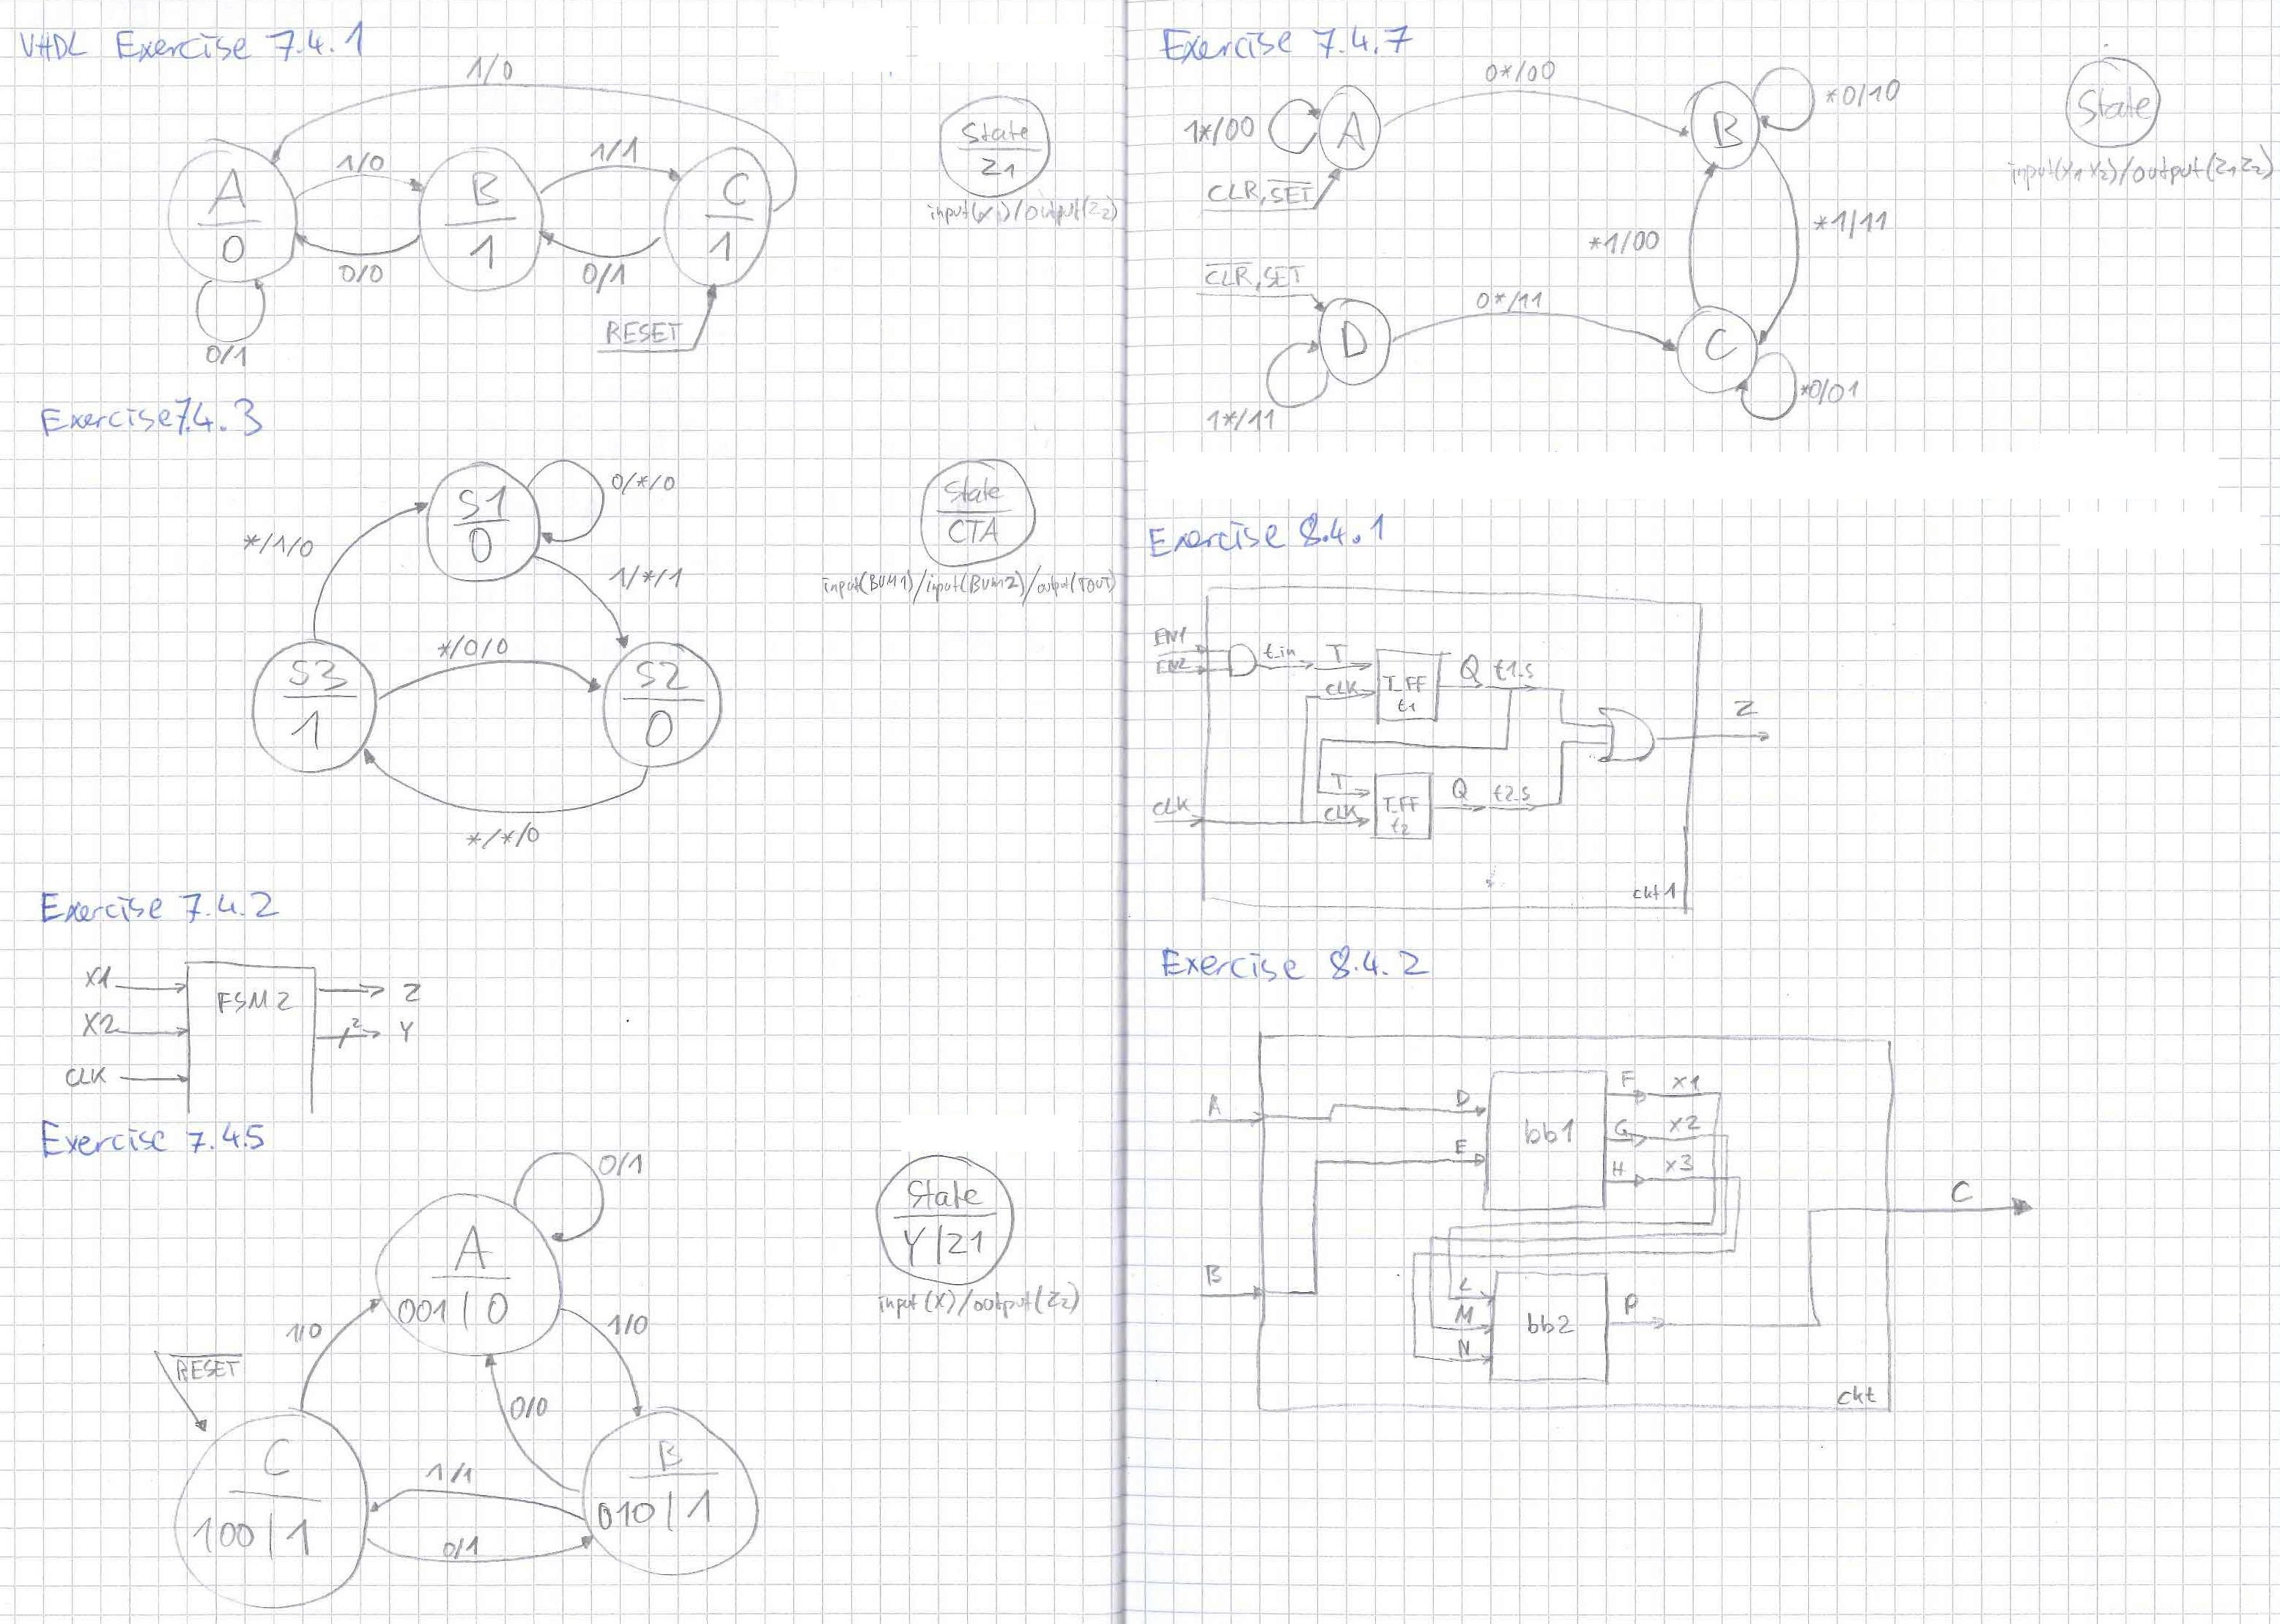
\includegraphics[width=0.5\textwidth, clip, trim={67 696 2524 1294}]{pics/solutions/chapter7+8_draft.jpg}

Basic source code to start with for solution:
\begin{lstlisting}[]
library IEEE;
use IEEE.std_logic_1164.all;
use IEEE.numeric_std.all;

entity FPGA_Chapter_7 is
	port
	(
		-- Input ports
		user_pb    : in std_logic_vector (0 to 2);
		clkin_50   : in std_logic;

		-- Output ports
		user_led   : out std_logic_vector (0 to 3) := "1111"
	);
end FPGA_Chapter_7;

architecture archi of FPGA_Chapter_7 is
	signal output  : std_logic := '0';
	signal clk_1Hz : std_logic := '0';
	
	type state_type is (Sa,Sb,Sc);
	signal PS, NS         : state_type;
	signal X1, X2, CLK, Z : std_logic := '0';
	signal Y              : std_logic_vector(1 downto 0) := "10";

begin

	process(clkin_50) is
		variable clk_counter : integer := 0;
	begin
		if(rising_edge(clkin_50)) then
			clk_counter := clk_counter + 1;

			if(clk_counter mod 25000000 = 0) then
				clk_1Hz <= NOT clk_1Hz;
			end if;

			if(clk_counter = 50000000) then
				clk_counter := 0;
			end if;
		end if;
	end process;

	X1 <= NOT user_pb(0);
	X2 <= NOT user_pb(1);
	CLK <= clk_1Hz;

	sync_p: process (CLK,NS)
	begin
		if (rising_edge(CLK)) then
			PS <= NS;
		end if;
	end process sync_p;	
	
	comb_p: process (CLK,X1,X2)
	begin
		case PS is
			when Sa =>
				Y <= "10";
				Z <= '0';
				if(X1 = '0') then
					NS <= Sa;
				else
					NS <= Sc;
				end if;
			when Sb =>
				Y <= "11";
				if(X2 = '0') then
					Z <= '1';
					NS <= Sa;
				else
					Z <= '0';
					NS <= Sb;
				end if;
			when Sc =>
				Y <= "01";
				if(X2 = '0') then
					Z <= '1';
					NS <= Sa;
				else
					Z <= '0';
					NS <= Sb;
				end if;
		end case;
	end process comb_p;
	
	user_led <= NOT (Y & Z & clk_1Hz);
end archi;
\end{lstlisting}

\subsection*{Exercise 3}
% TODO: draw solution from draft
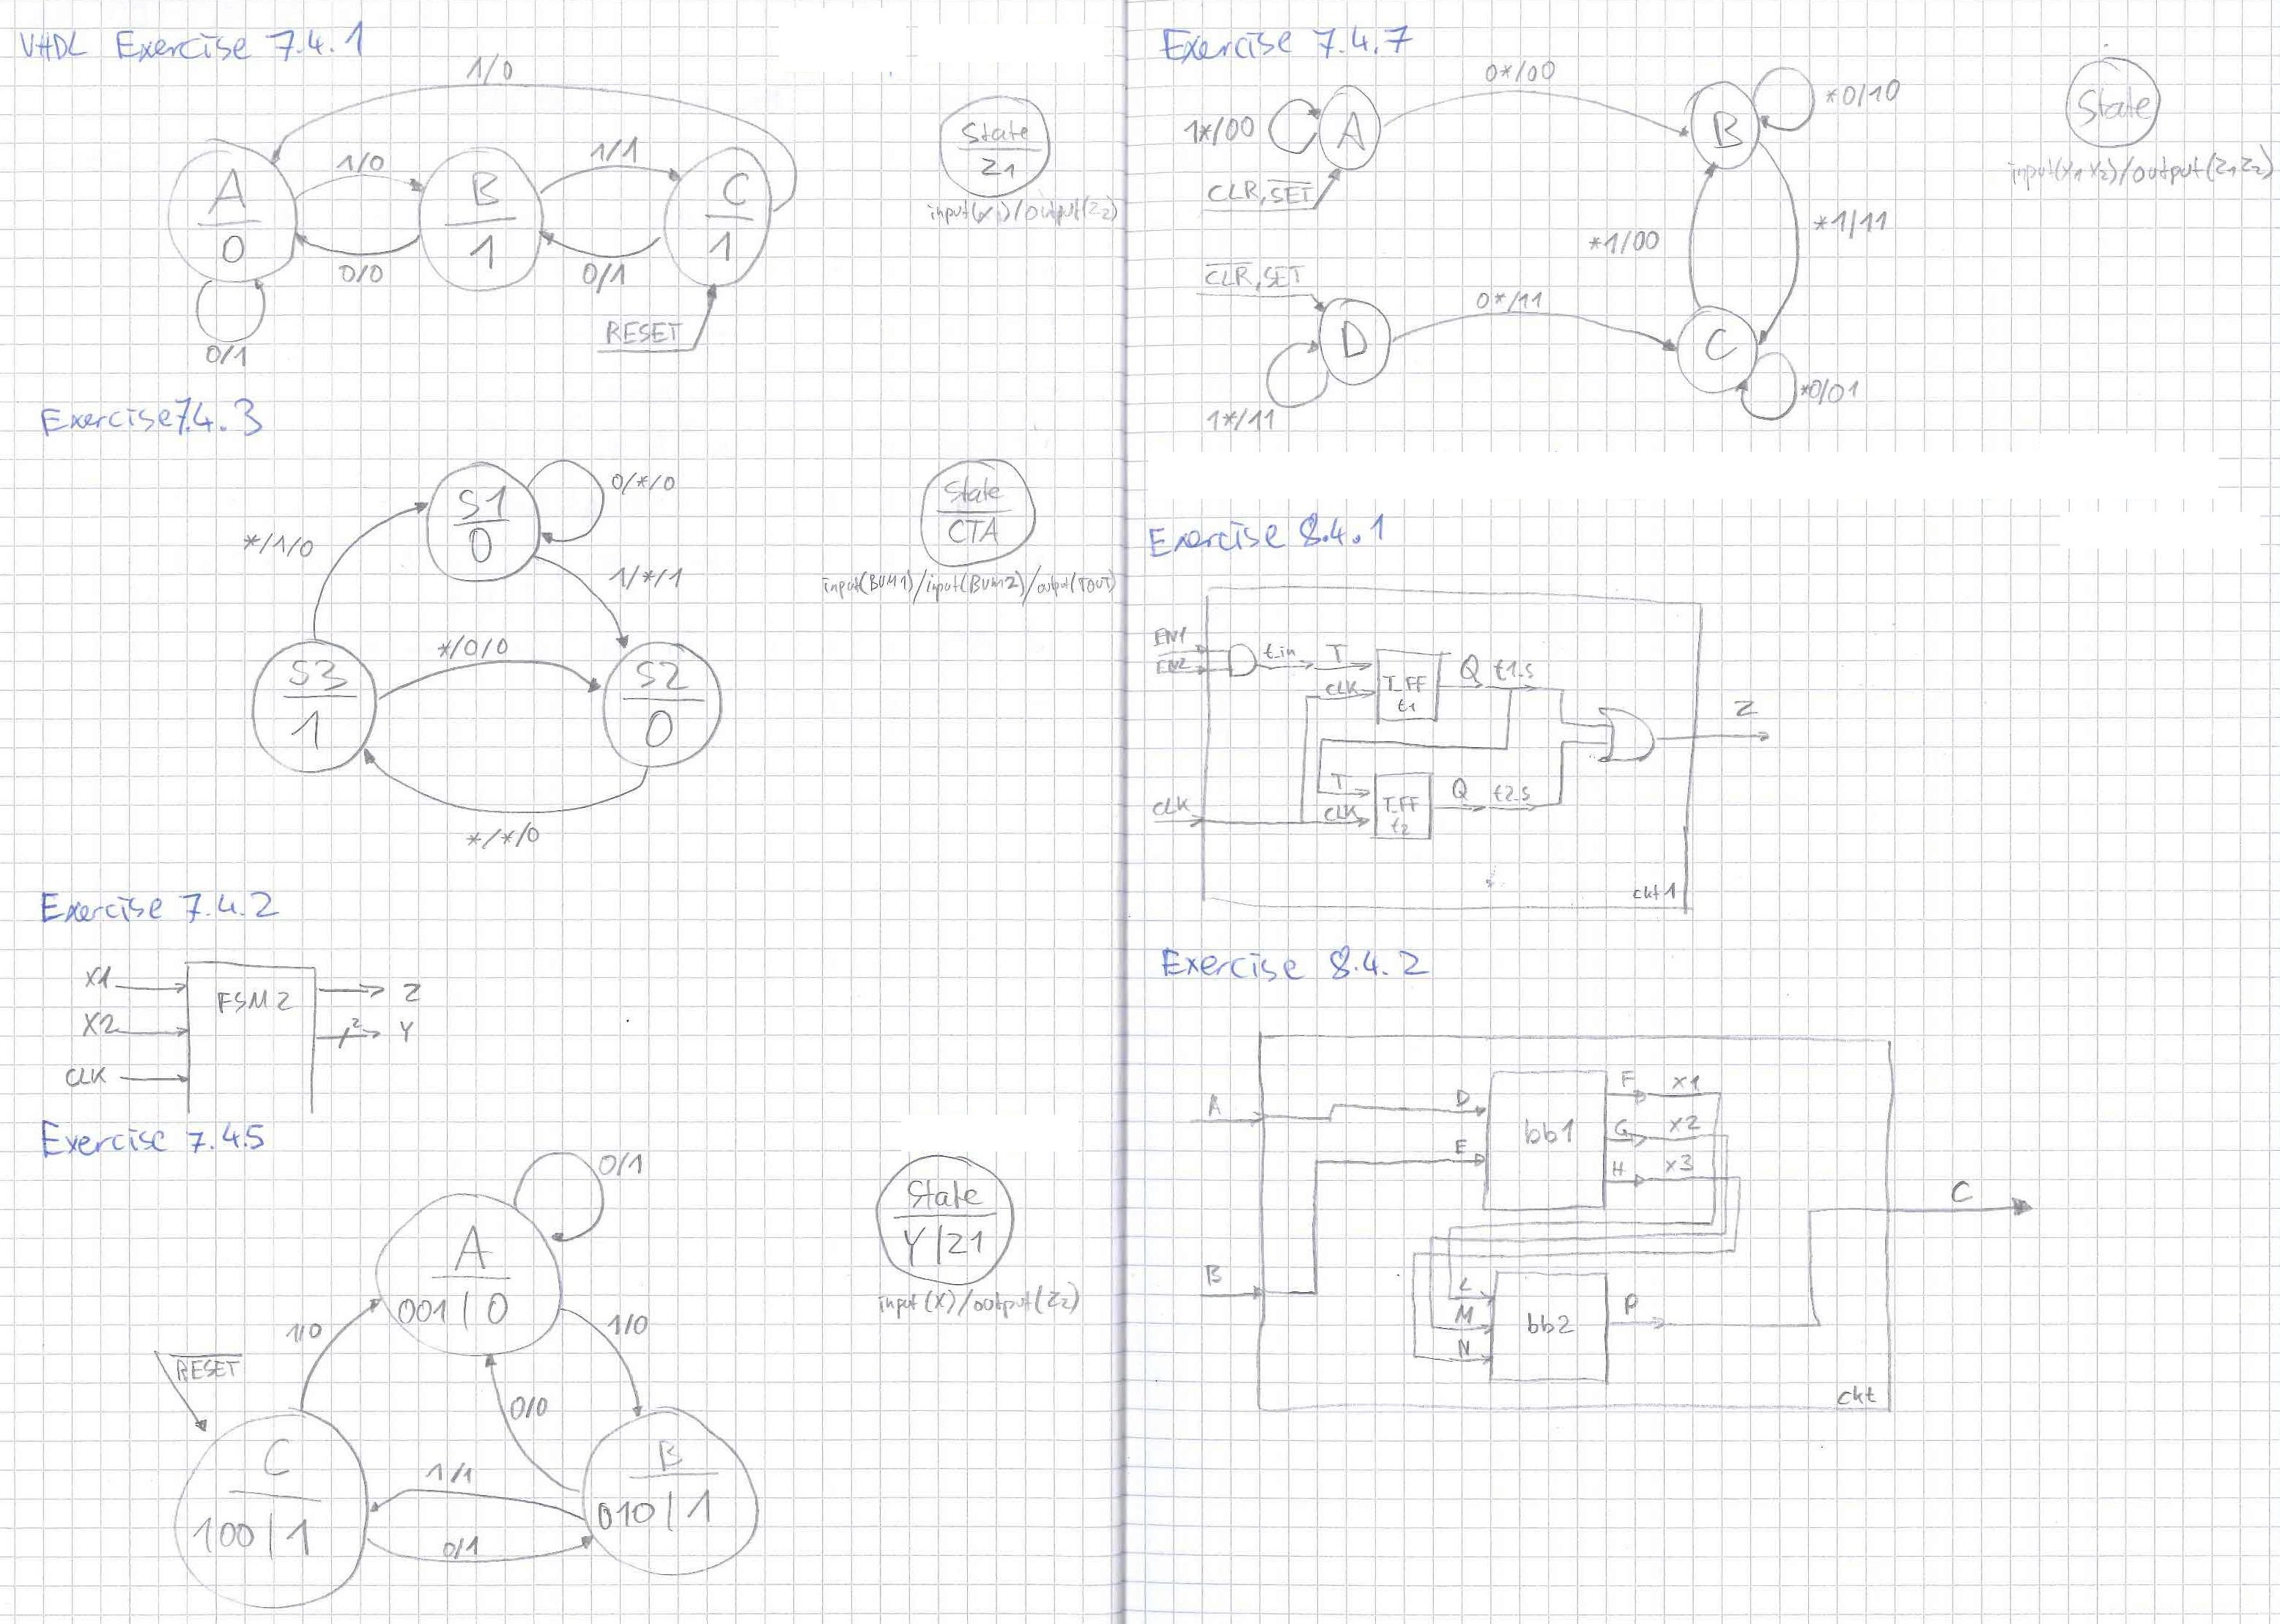
\includegraphics[width=\textwidth, clip, trim={319 1045 1581 610}]{pics/solutions/chapter7+8_draft.jpg}

\subsection*{Exercise 4}
% TODO: Write solutions

\subsection*{Exercise 5}
% TODO: draw solution from draft
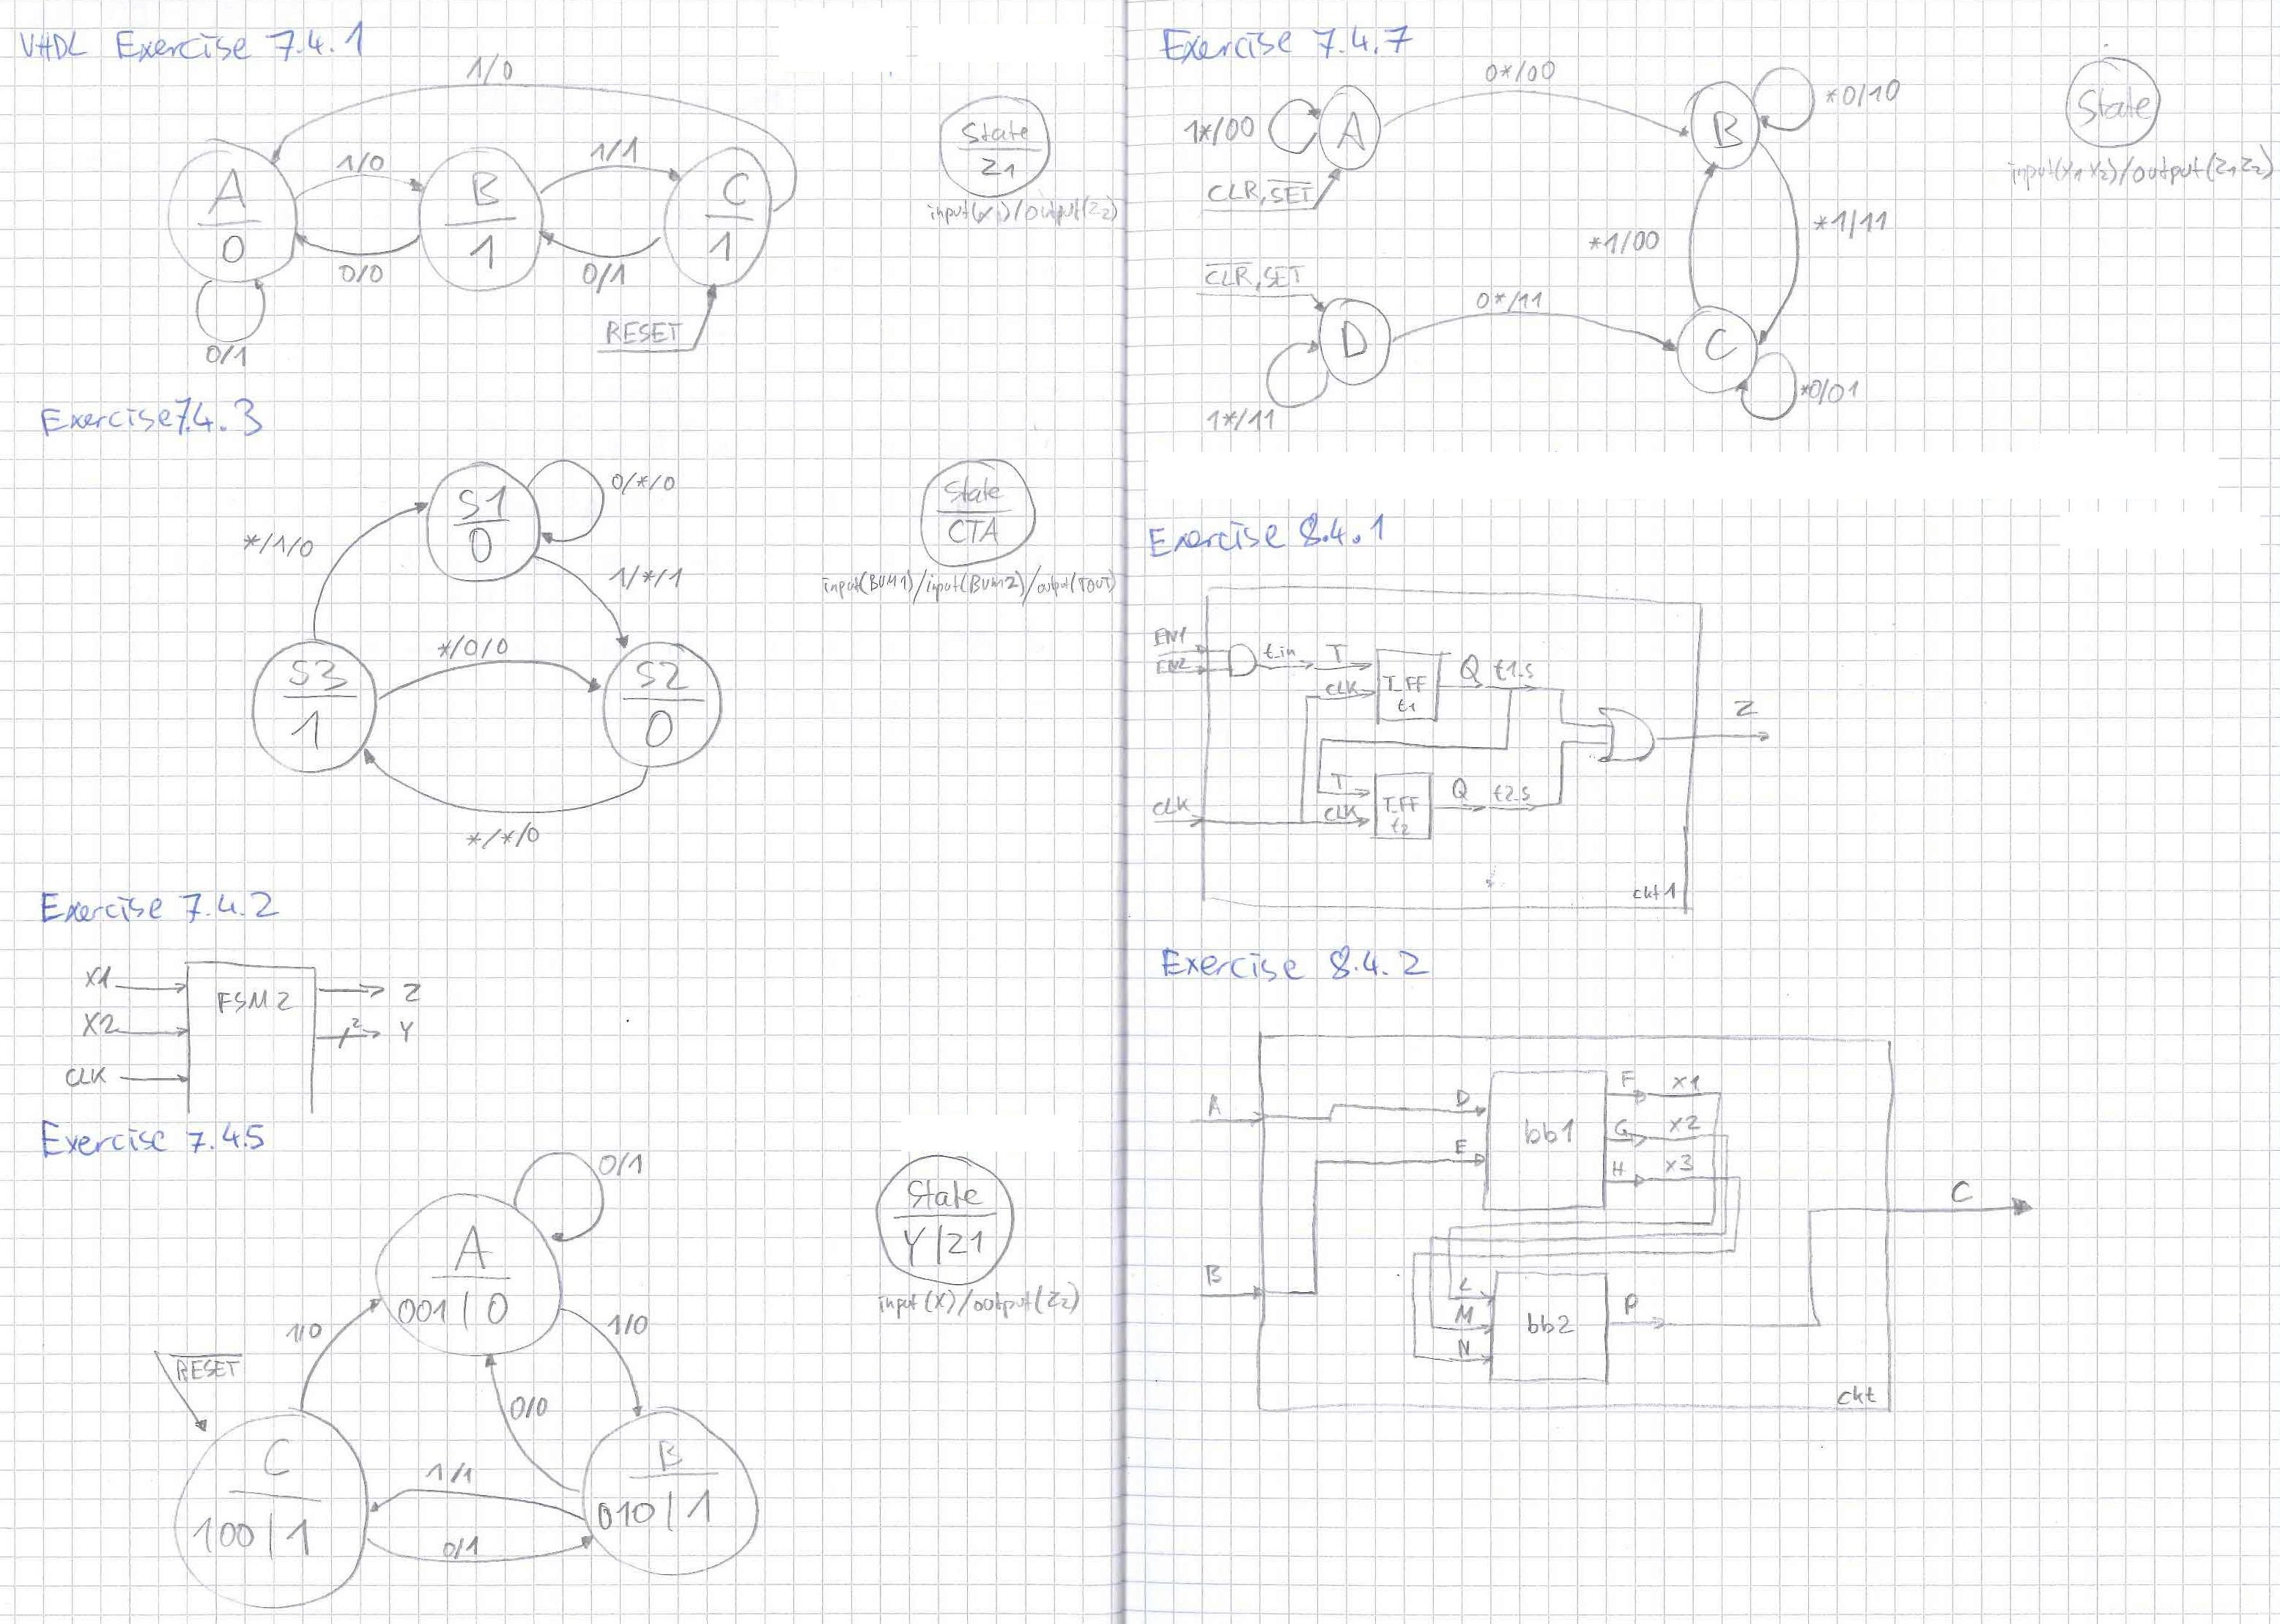
\includegraphics[width=\textwidth, clip, trim={184 13 1631 1571}]{pics/solutions/chapter7+8_draft.jpg}

\subsection*{Exercise 6}
% TODO: Write solutions

\subsection*{Exercise 7}
% TODO: draw solution from draft
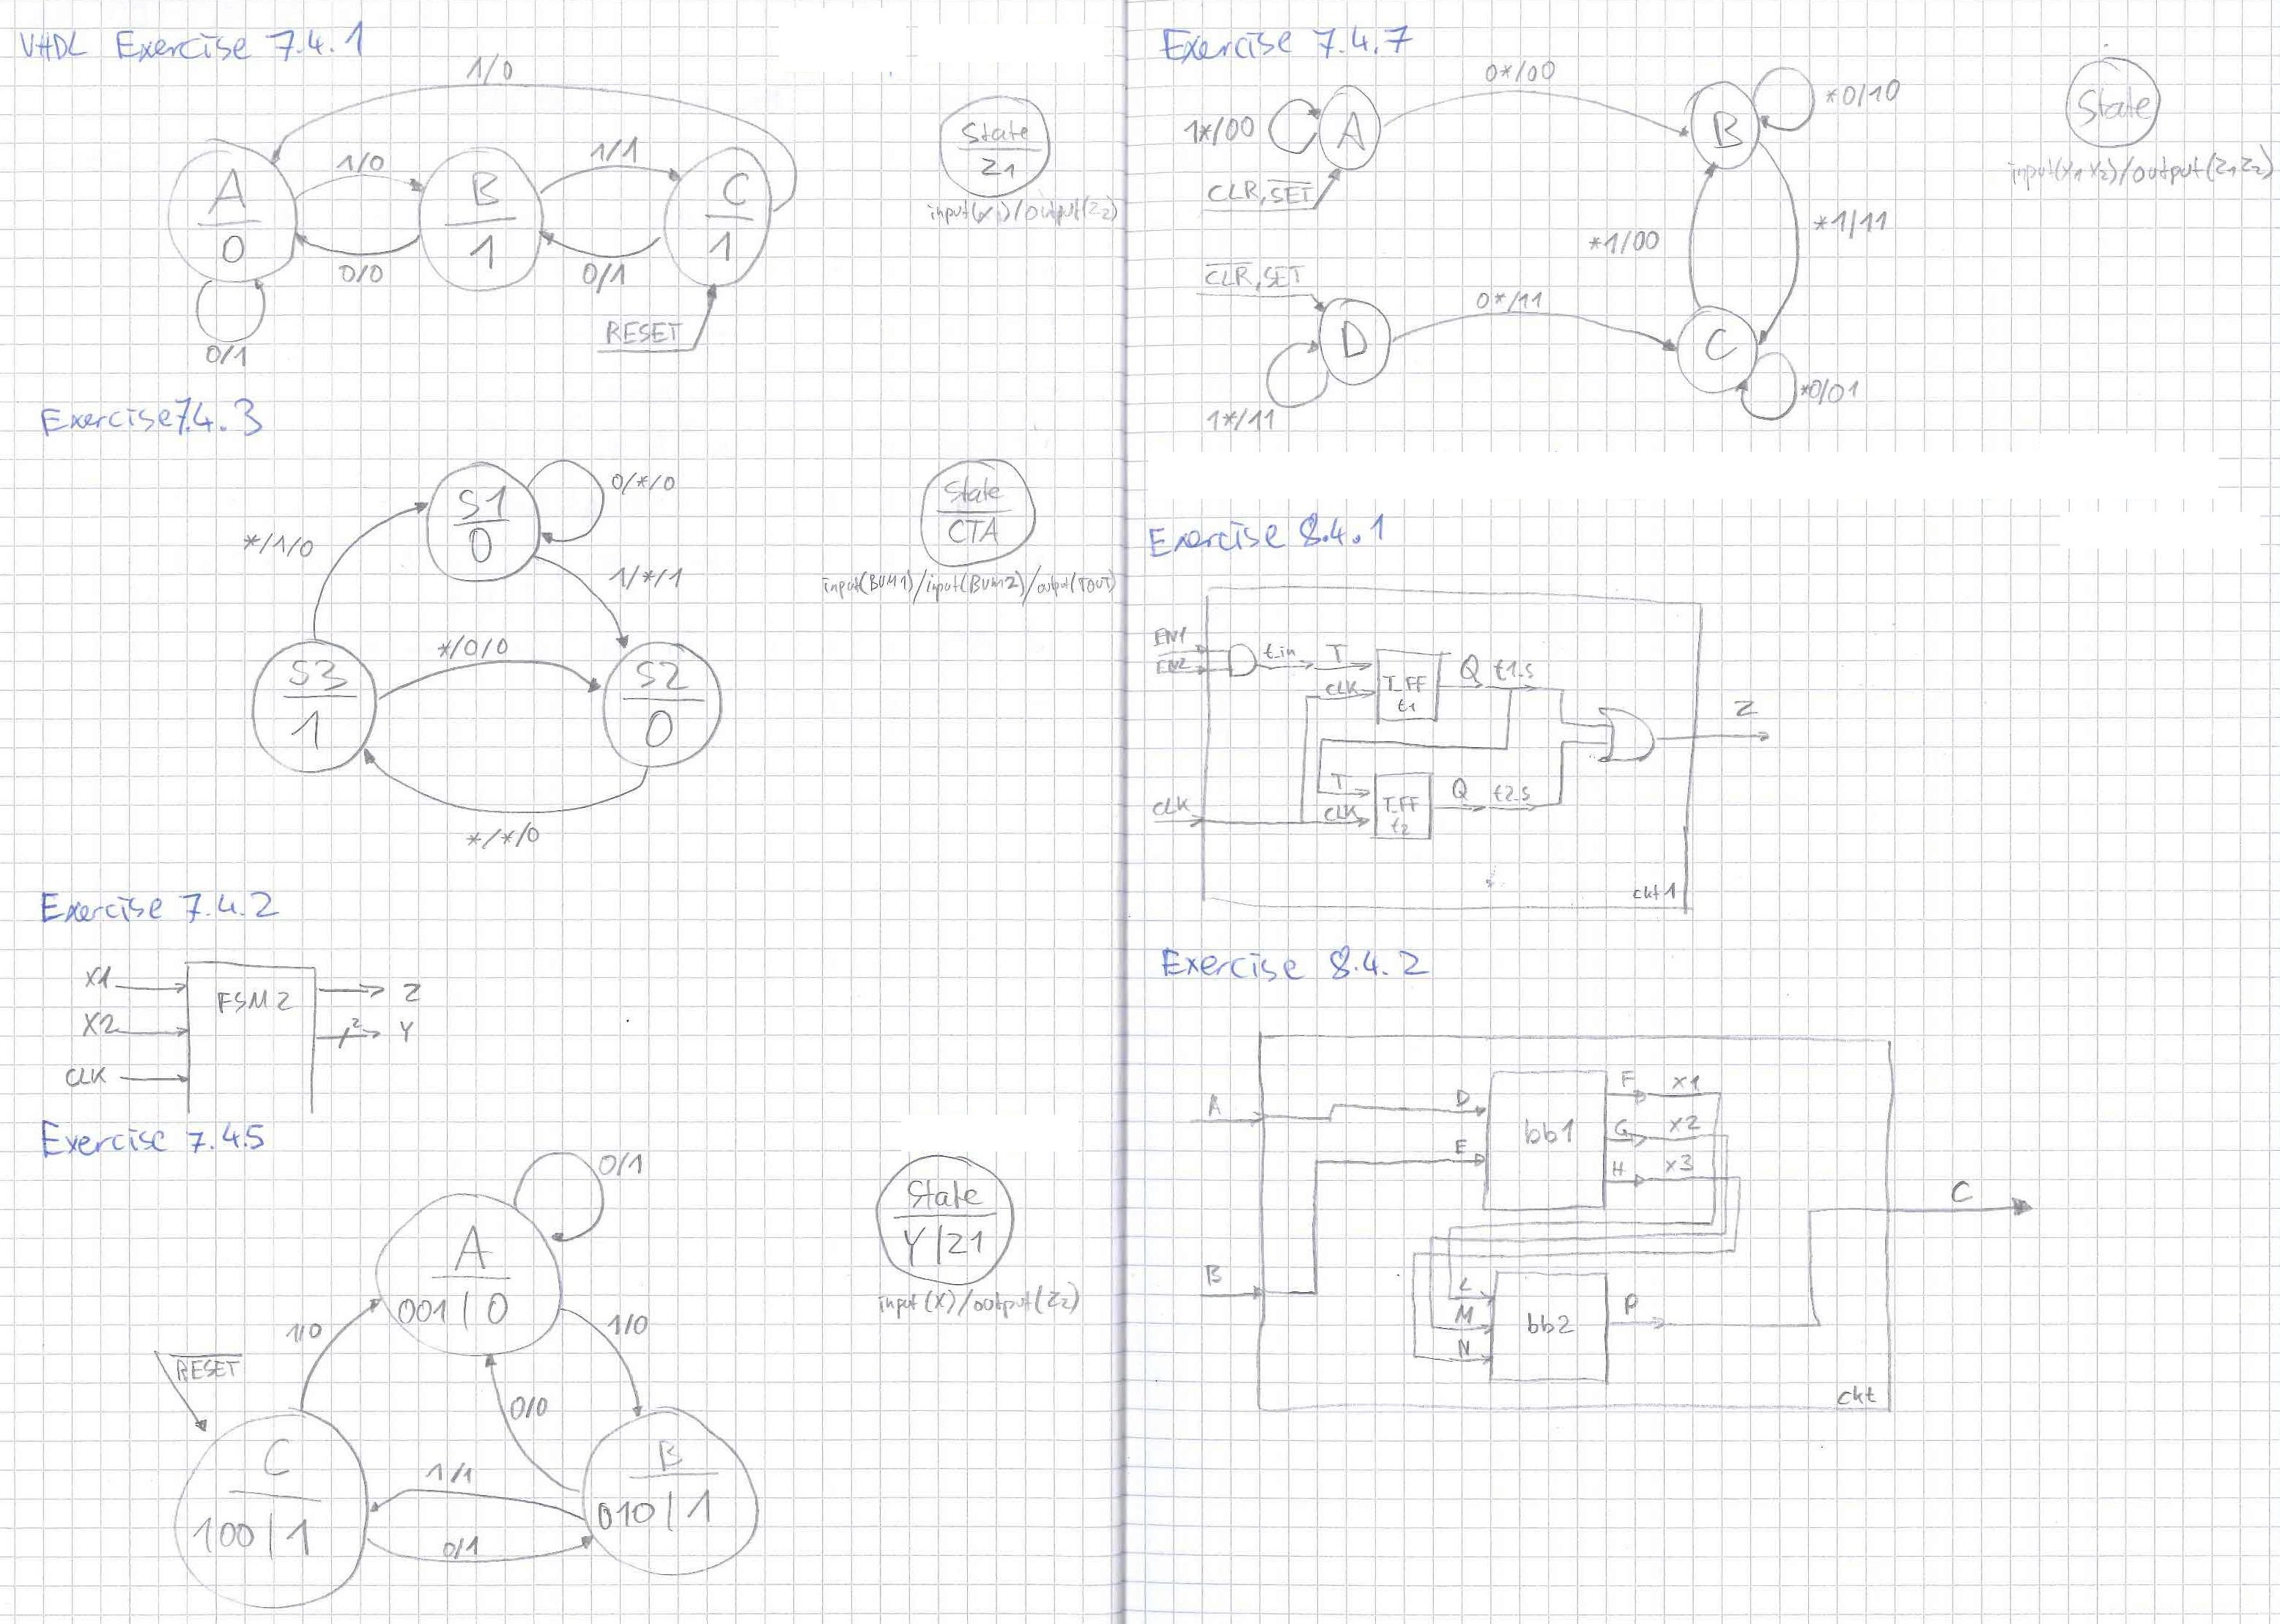
\includegraphics[width=\textwidth, clip, trim={1608 1624 5 72}]{pics/solutions/chapter7+8_draft.jpg}

\subsection*{Exercise 8}
% TODO: Write solutions

\subsection*{Exercise 9}
% TODO: Write solutions

\subsection*{Exercise 10}
% TODO: Write solutions

\subsection*{Exercise 11}
% TODO: Write solutions

\subsection*{Exercise 12}
% TODO: Write solutions

\subsection*{Exercise 13}
% TODO: Write solutions

\subsection*{Exercise 14}
% TODO: Write solutions

\section{Solutions \ref{structural_modeling_in_vhdl_exercises}~\nameref{structural_modeling_in_vhdl_exercises}}
\subsection*{Exercise 1}
% TODO: draw solution from draft
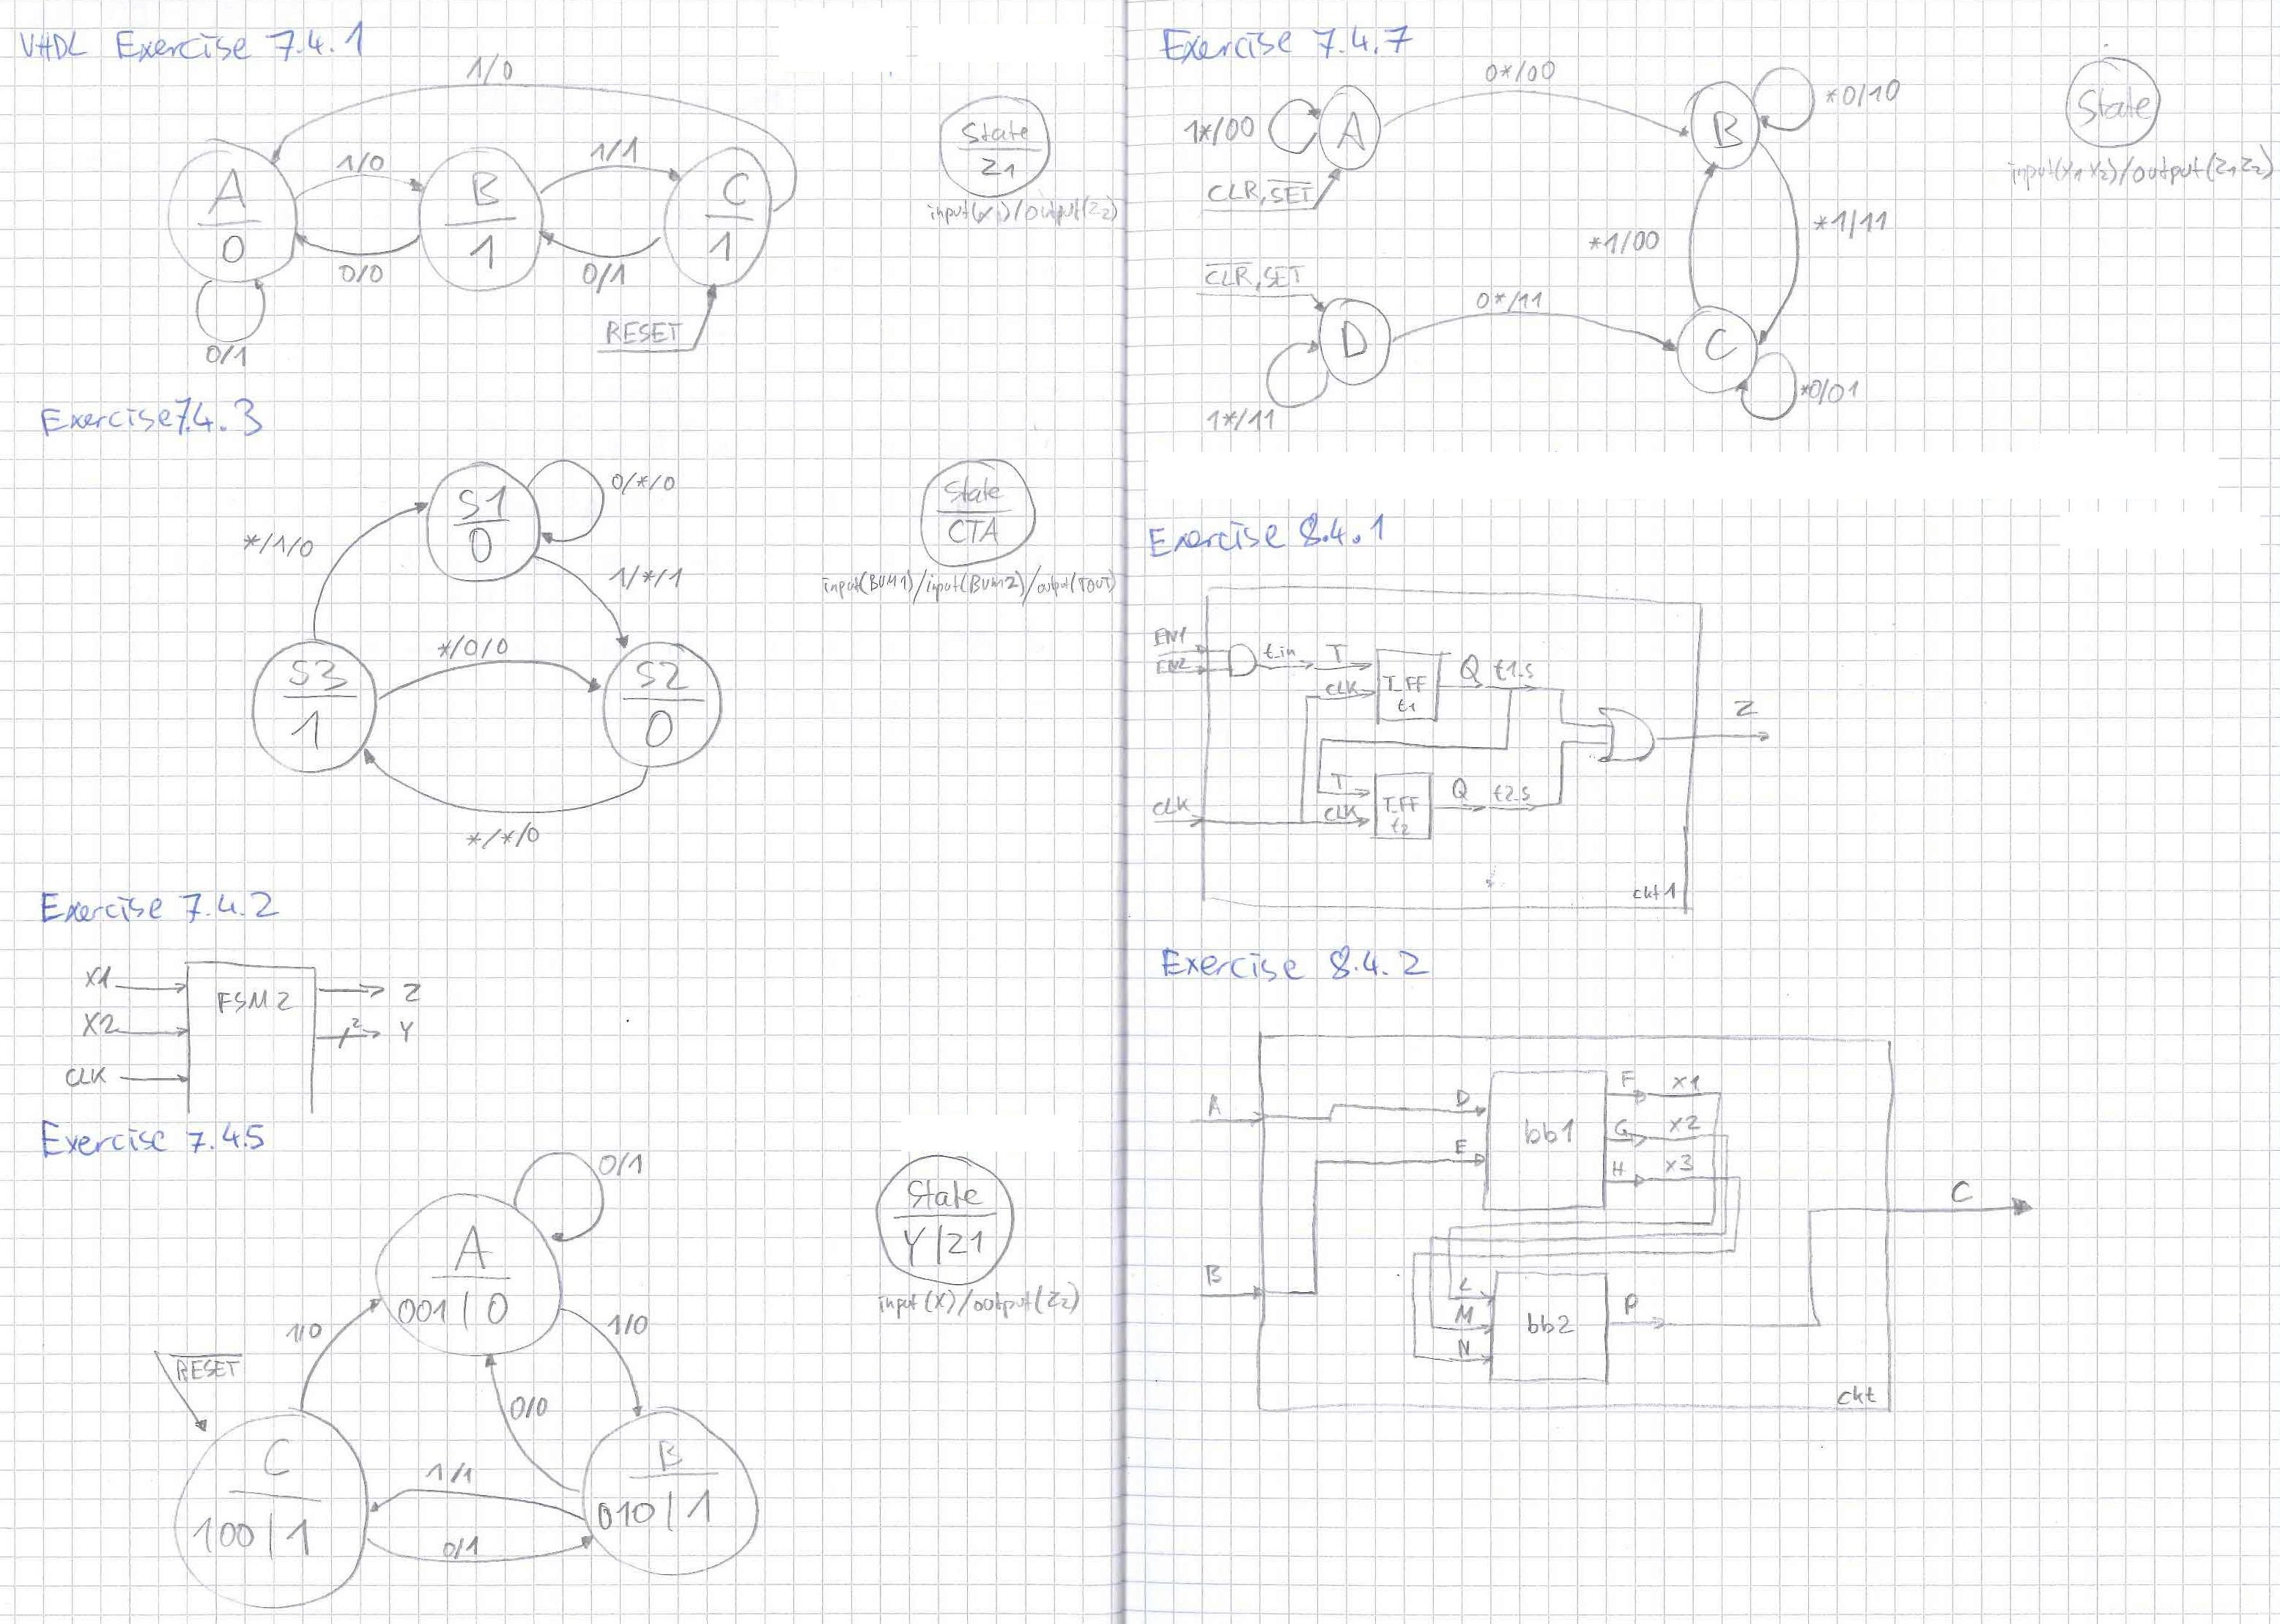
\includegraphics[width=\textwidth, clip, trim={1563 958 681 790}]{pics/solutions/chapter7+8_draft.jpg}

\subsection*{Exercise 2}
% TODO: draw solution from draft
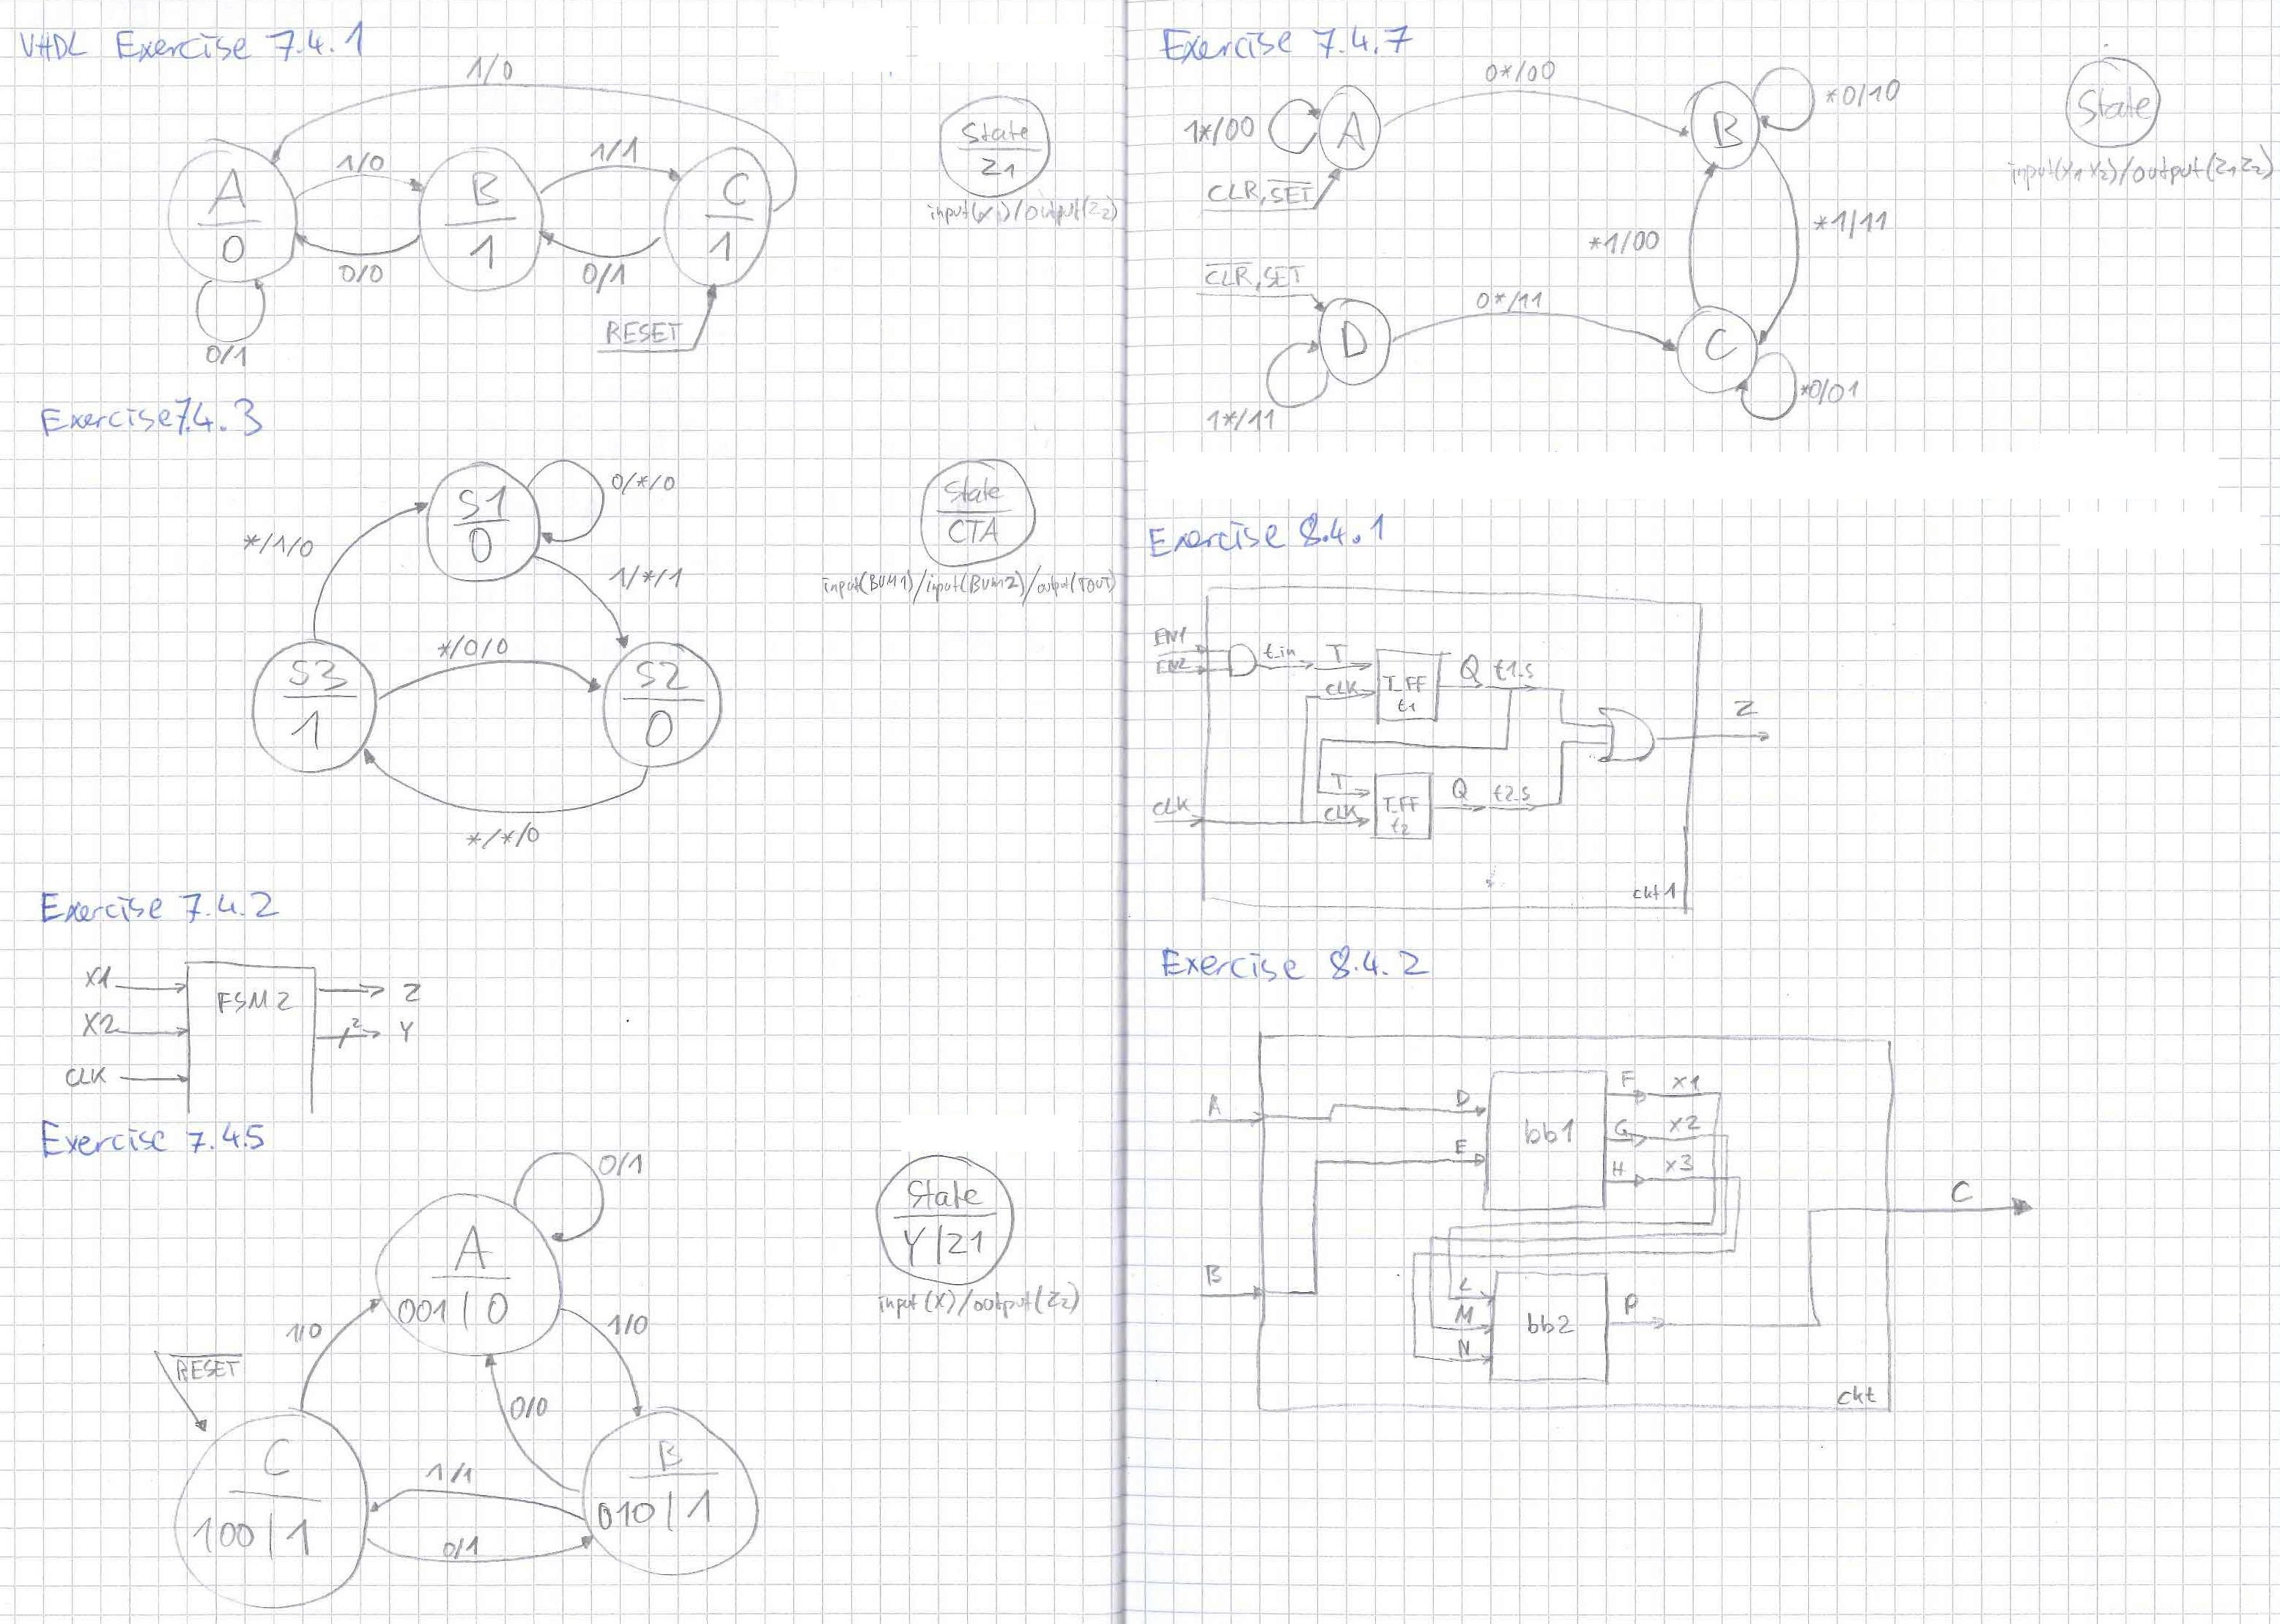
\includegraphics[width=\textwidth, clip, trim={1618 275 332 1394}]{pics/solutions/chapter7+8_draft.jpg}

\subsection*{Exercise 3}
% TODO: write solution from example source (working vhdl code)
a) Basic source code to start with for solution:

\begin{lstlisting}[]
library IEEE;
use IEEE.std_logic_1164.all;

entity FPGA_Chapter_8 is
	port
	(
		-- Input ports
		user_pb    : in std_logic_vector (0 to 2);

		-- Output ports
		user_led   : out std_logic_vector (0 to 3) := "1111"
	);
end FPGA_Chapter_8;

library IEEE;
use IEEE.std_logic_1164.all;

---------------------------------
-- Description of AND function --
---------------------------------
entity my_and is
	port
	(
		A, B : in  std_logic;
		F    : out std_logic
	);
end my_and;

architecture ckt_and of my_and is
begin
	F <= (A and B);
end ckt_and;

library IEEE;
use IEEE.std_logic_1164.all;

--------------------------------
-- Description of OR function --
--------------------------------
entity my_or is
	port
	(
		A, B : in  std_logic;
		F    : out std_logic
	);
end my_or;

architecture ckt_or of my_or is
begin
	F <= (A or B);
end ckt_or;

architecture archi of FPGA_Chapter_8 is
	signal output : std_logic := '0';

	signal A, B, C, D, F : std_logic := '0';
	signal and1out, and2out : std_logic := '0';

	-- 2-input AND gate -------------
	component my_and is
		port(
			A, B : in  std_logic;
			F    : out std_logic
		);
	end component;

	-- 2-input OR gate --------------
	component my_or is
		port(
			A, B : in  std_logic;
			F    : out std_logic
		);
	end component;

begin
	A <= not user_pb(0);
	B <= not user_pb(1);
	C <= not user_pb(2);

	-- Chapter 8.4.3 a)
	and1: my_and port map(A => A,       B => not B,   F => and1out);
	and2: my_and port map(A => not A,   B => not C,   F => and2out);
	or1:  my_or  port map(A => and1out, B => and2out, F => F);

	user_led(0) <= not F;
end archi;
\end{lstlisting}


b) % TODO: write example

c) % TODO: write example

d) % TODO: write example

\section{Solutions \ref{registers_and_register_transfer_level_exercises}~\nameref{registers_and_register_transfer_level_exercises}}
\subsection*{Exercise 1}
% TODO: Write solutions

\subsection*{Exercise 2}
% TODO: Write solutions

\subsection*{Exercise 3}
% TODO: Write solutions

\subsection*{Exercise 4}
% TODO: Write solutions

\subsection*{Exercise 5}
% TODO: Write solutions

\subsection*{Exercise 6}
% TODO: Write solutions

